\documentclass[fleqn]{exam}
\usepackage{amsmath,amsthm,amssymb}
\usepackage{tasks}
\usepackage{enumitem}
\usepackage{graphicx}
\usepackage{tikz}
\usepackage{multicol}
\usepackage{wrapfig}

\rhead{Robert Smith - \today}
\lhead{Otis C - Lesson 20 Questions}

\begin{document}

\section*{Functions and Graphs}

\begin{questions}

\question Hello

\begin{parts}
\part answer 1
\part answer 2
\end{parts}

\question Fill in the following tables and graph on the same axis.

\begin{multicols}{2}

\begin{tabular}{|l|c|c|c|c|c|c|c|c|}
\hline 
$x$ & 0 & 1 & 2 & 3 & 4 & 5 & 6 & 7 \\
\hline 
$y$ & & 1 & 3 &  &  &  & 11 & 13 \\
\hline
\end{tabular}

\begin{tabular}{|l|c|c|c|c|c|c|c|c|}
\hline 
$x$ & 0 & 1 & 2 & 3 & 4 & 5 & 6 & 7 \\
\hline 
$y$ & & 1 & 3 &  &  &  & 11 & 13 \\
\hline 
\end{tabular}

\begin{tabular}{|l|c|c|c|c|c|c|c|c|}
\hline 
$x$ & 0 & 1 & 2 & 3 & 4 & 5 & 6 & 7 \\
\hline 
$y$ & & 1 & 3 &  &  &  & 11 & 13 \\
\hline 
\end{tabular}
	
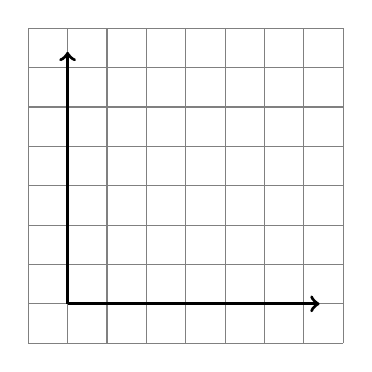
\begin{tikzpicture}
\draw[step=0.5cm,color=gray] (0,0) grid (4,4);
\draw[color=black,very thick,->] (0.5,0.5) -- (0.5,3.7);
\draw[color=black,very thick,->] (0.5,0.5) -- (3.7,0.5);
\end{tikzpicture}

\end{multicols}

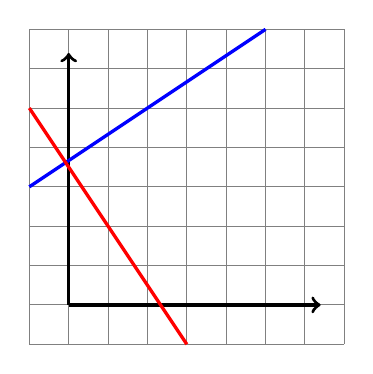
\begin{tikzpicture}
\draw[step=0.5cm,color=gray] (0,0) grid (4,4);
\draw[color=black,very thick,->] (0.5,0.5) -- (0.5,3.7);
\draw[color=black,very thick,->] (0.5,0.5) -- (3.7,0.5);
\draw[color=blue,very thick,-] (0,2) -- (3,4);
\draw[color=red,very thick,-] (0,3) -- (2,0);
\end{tikzpicture}


%\begin{wrapfigure}{r}{\textwidth}
%
%\begin{tikzpicture}
%\draw[step=0.5cm,color=gray] (0,0) grid (4,4);
%\draw[color=black,very thick,->] (0.5,0.5) -- (0.5,3.7);
%\draw[color=black,very thick,->] (0.5,0.5) -- (3.7,0.5);
%\end{tikzpicture}
%
%\end{wrapfigure}
%
%\begin{wrapfigure}{R}{\textwidth}
%
%\includegraphics[width=0.48\textwidth]{grid}
%
%\end{wrapfigure}






\end{questions}






\end{document}
